\documentclass[%
 reprint,
%superscriptaddress,
%groupedaddress,
%unsortedaddress,
%runinaddress,
%frontmatterverbose, 
%preprint,
%showpacs,preprintnumbers,
%nofootinbib,
%nobibnotes,
%bibnotes,
 amsmath,amssymb,
 aps,
%pra,
%prb,
%rmp,
%prstab,
%prstper,
%floatfix,
]{revtex4-1}

\usepackage{graphicx}% Include figure files
\usepackage{dcolumn}% Align table columns on decimal point
\usepackage{bm}% bold math
%\usepackage{hyperref}% add hypertext capabilities
%\usepackage[mathlines]{lineno}% Enable numbering of text and display math
%\linenumbers\relax % Commence numbering lines

%\usepackage[showframe,%Uncomment any one of the following lines to test 
%%scale=0.7, marginratio={1:1, 2:3}, ignoreall,% default settings
%%text={7in,10in},centering,
%%margin=1.5in,
%%total={6.5in,8.75in}, top=1.2in, left=0.9in, includefoot,
%%height=10in,a5paper,hmargin={3cm,0.8in},
%]{geometry}

\begin{document}

%\preprint{APS/123-QED}

\title{Nuclear astrophysical implications of a reduction in the fine structure constant}% 
\thanks{Midterm paper for PHYS-554: Nuclear Astrophysics}%

\author{Adam Richie-Halford}
\email{richford@uw.edu}
\affiliation{
 Department of Physics \\
 University of Washington \\
 Seattle, Washington 98195, USA
}

\date{\today}% It is always \today, today,
             %  but any date may be explicitly specified

\begin{abstract}
An article usually includes an abstract, a concise summary of the work
covered at length in the main body of the article. 
%\begin{description}
%\item[Usage]
%Secondary publications and information retrieval purposes.
%\item[Structure]
%You may use the \texttt{description} environment to structure your abstract;
%use the optional argument of the \verb+\item+ command to give the category of each item. 
%\end{description}
\end{abstract}

\pacs{Valid PACS appear here}% PACS, the Physics and Astronomy
                             % Classification Scheme.
%\keywords{Suggested keywords}%Use showkeys class option if keyword
                              %display desired
\maketitle

%\tableofcontents

\section{\label{sec:intro}Introduction}

The recent discover of a parallel universe\cite{ReddyMidterm} has spurred speculation about its nuclear astrophysical properties. Remarkably, this parallel universe has identical fundamental constants $\hbar$ and $c$ as well as identical parameters of QCD and of the weak interactions. The quark and lepton masses are also identical. The only difference in fundamental constants is that of the fine structure constant, which in the parallel universe is given by
\begin{equation}
	\widetilde{\alpha} = \alpha / 2 = 1 / 274.
\end{equation}
This reduction in $\alpha$ also alters the neutron-proton mass difference, which is given by\cite{ReddyMidterm}
\begin{equation}
	\Delta \widetilde{m} = \widetilde{m_n} - \widetilde{m_p} \approx 2 \; \text{MeV}.
\end{equation}

I will discuss the implications of this reduction in $\alpha$. In Section \ref{sec:masses}, I discuss the effect on nuclear masses and calculate the $A$ and $Z$ numbers of the most stable nucleus using the

\section{\label{sec:conclusion}Results}

\subsection{\label{sec:masses}Effects on nuclear masses}

\subsubsection{\label{sec:table_of_nuclides}Nuclide stability}

Ignoring shell effects and pairing effects, one may approximate the binding energy of a nucleus using the Weizs\"acker mass formula\cite{1935ZPhy...96..431W}
\begin{equation}
    B(A, Z) = a_V A - a_S A^{2/3} - a_C \frac{Z (Z-1)}{A^{1/3}}
    - a_{\text{sym}} \frac{(N-Z)^2}{A}.
    \label{eq:weizsacker}
\end{equation}

The volume and surface terms are based on the strong nuclear force, so they should remain unchanged in the parallel universe. Using one popular set of values for the Weizs\"acker coefficients\cite{wong1990introductory}, we may take
\begin{equation}
    a_V = 16 \; \text{MeV} \\
    a_S = 17 \; \text{MeV}.
\end{equation}
Similarly, the symmetry term is not based on the fundamental forces but rather on the Pauli exclusion principle. So we may use the value of $a_{\text{sym}} = 25 \; \text{MeV}$ to be the same as in our universe.\cite{wong1990introductory}

In our universe, $a_C = 0.6 \; \text{MeV}$. We can approximate $a_C$ by equating it with the energy of a charged sphere,
\begin{equation}
    \frac{3}{5} \frac{Z^2 e^2}{4 \pi \epsilon_0 R} = 
    \frac{3}{5} \frac{Z^2 \alpha \hbar c}{R}
    \approx a_C \frac{Z(Z-1)}{A^{1/3}}.
\end{equation}

So if the value of the fine structure constant were reduced by one-half, then the Coulomb term in the mass formula would also be reduced by the same amount,
\begin{equation}
    \alpha \rightarrow \widetilde{\alpha} = \frac{\alpha}{2}
    \quad \Longrightarrow \quad
    a_C \rightarrow \widetilde{a}_C = \frac{a_C}{2}.
\end{equation}
Thus, in the parallel universe, we have $\widetilde{a}_C = 0.3 \; \text{MeV}$.

To gain intuition about the differences between our universes, I plot the nuclide valley of stability by plotting a contour of the neutron and proton drip lines using the mass formula in Eq\eqref{eq:weizsacker}. The drip lines will be determined by the point at which the separation energies $S_p$ and $S_n$ vanish,
\begin{align}
	S_n &= E_B(N+1, Z) - E_B(N, Z) = 0, \\
	S_p &= E_B(N, Z+1) - E_B(N, Z) = 0.
\end{align}
In the region of stability, $S_n S_p > 0$, so we may plot contour lines of the quantity $S_n S_p$ and restrict to positive values to visualize the table of nuclides. In Figure \ref{fig:nuclides}, I use this technique to plot the stable nuclides for $0 < N < 100$ and $0 < Z < 100$, both for our universe and for ``their" universe.

\begin{figure}[h!]
\centering
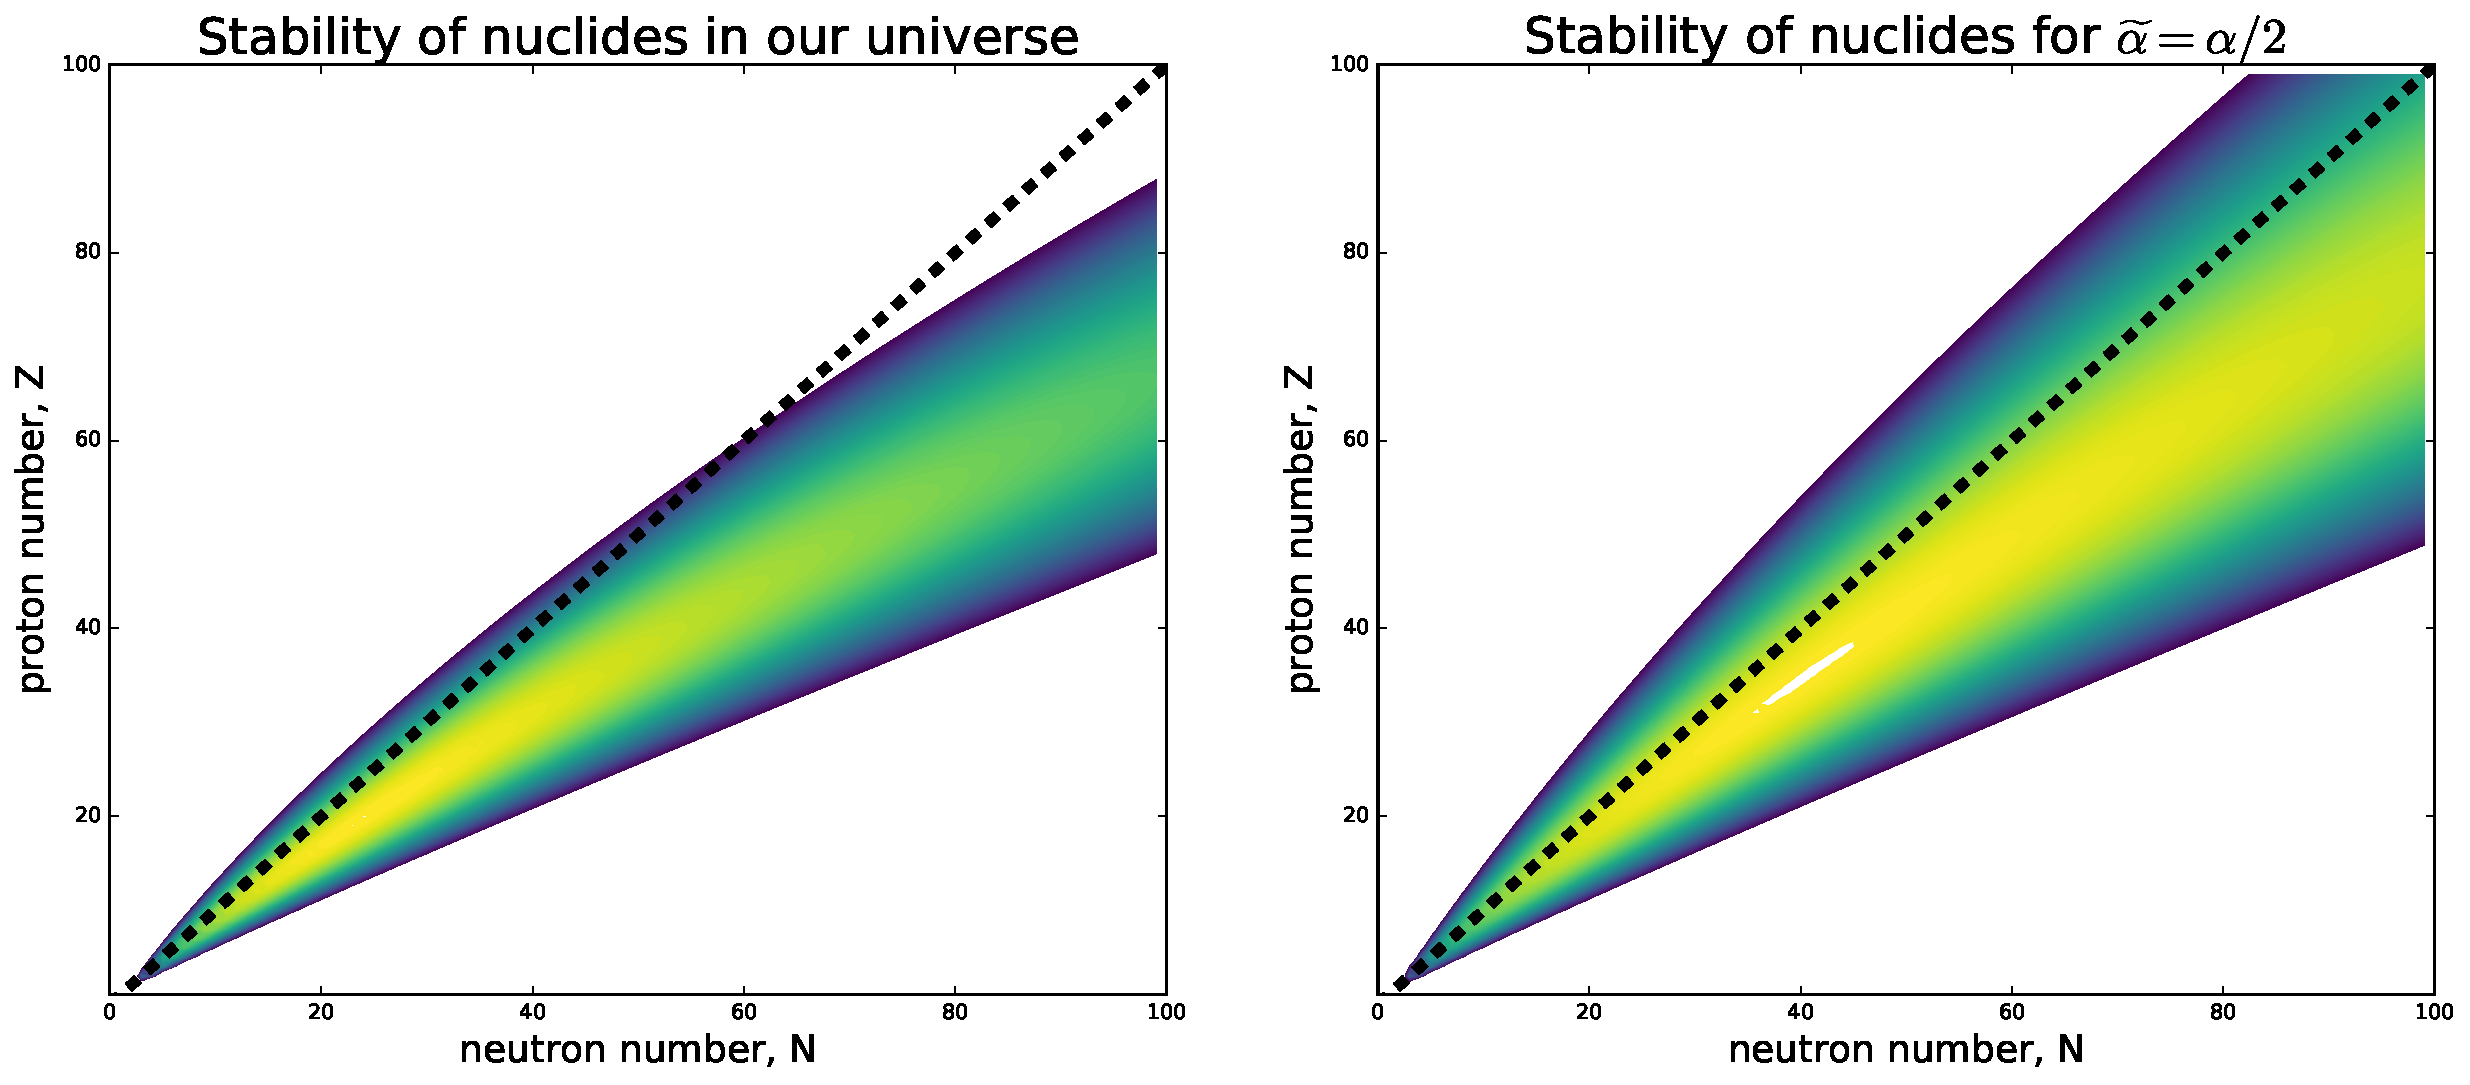
\includegraphics[width=\linewidth]{fig/nuclides.pdf}
\caption{\label{fig:nuclides}Table of nuclides in our universe (left) and ``their" universe (right). I plot a contour of $S_n S_p$ to visualize the valley of stability in both universes. The dotted black line shows the $A=Z$ reference line. In our universe, larger nuclei have higher proton-neutron asymmetry in order to compensate for Coulomb repulsion. As expected, in the parallel universe, nuclides have similar numbers of protons and neutrons due to the reduced proton charge.}
\end{figure}

The parallel universe's valley of stability follows the $A=Z$ reference line much more closely than in our universe. This is as expected, since the reduction in $\alpha$ reduces the proton charge, and therefore the Coulomb repulsion inside each nucleus.

\subsubsection{\label{sec:stable_nuclei}Identifying stable nuclei}

For a fixed nucleon number, A, one can find the optimal proton number by maximizing the binding energy
\begin{equation}
    \left. \frac{d E_b}{d Z}\right|_{\text{fixed A}} =
    - a_C \frac{2Z - 1}{A^{1/3}}
    + a_{\text{sym}} \frac{4 (A - 2Z)}{A}
    \overset{!}{=} 0.
\end{equation}

Solving this equation for $Z$ and inserting into Eq\eqref{eq:weizsacker} yields an equation for the binding energy as a function of $A$ only. I then solve this equation numerically to find the $A$ value that maximizes the binding energy per nucleon $E_b(A) / A$.\cite{jupyter_notebook}. This yields the $A$ value of the most stable nucleus.

In our universe, the most stable nucleus has $A = 67$ with a binding energy per nucleon of 9.63 MeV. In ``their" universe, the most stable nucleus has $A = 117$ with a binding energy per nucleon of 10.79 MeV.

\subsection{\label{sec:bbn}Effects on big bang nucleosynthesis (BBN)}

In the early universe, for a given $\mu$ and $T$, the nucleon densities are given by\cite{ReddyLectureNotes}
\begin{align}
    n_n = 2 \left( \frac{m_n T}{2 \pi} \right)^{3/2}
    \exp\left( \frac{-m_n}{T} \right) \exp\left( \frac{\mu_n}{T} \right), \\
    n_p = 2 \left( \frac{m_p T}{2 \pi} \right)^{3/2}
    \exp\left( \frac{-m_p}{T} \right) \exp\left( \frac{\mu_p}{T} \right).
\end{align}

For $T \ge 0.7 \; \text{MeV}$, the weak reaction rates that exchange protons and neutrons are fast compared to the expansion rate of the universe, so the difference in neutron and proton chemical potentials is negligible compared to their mass difference. So we can approximate the neutron-proton number density ratio as
\begin{equation}
    \frac{n_n}{n_p} \approx \exp \left( \frac{- \Delta m}{T} \right),
\end{equation}
where $\Delta m = m_n - m_p$.\cite{ReddyLectureNotes}

In the early universe, the temperature is very hot and neutrons and protons are roughly equally numerous. As the temperature of the universe cools below $\Delta m$, free neutrons begin to decay at a rate faster than they are produced by weak reactions. So the neutron fraction decreases until "neutron-proton freeze-out," which occurs at a temperature where the rate of weak reactions is equal to the expansion rate of the universe,\cite{CAMPBELL1995429}
\begin{equation}
    \sqrt{G_N N} T_f^2 \sim H(T_f) = \Gamma_\text{weak} (T_f) \sim G_F^2 T_f^5.
\end{equation}

Since the alternate universe has the same expansion rate and weak interaction parameters as our universe, we may take $T_f$ to be the same that is in our universe ($T_f = 0.7\; \text{MeV}$).

After freeze-out, we can approximate the neutron-proton number density ratio as fixed. This ratio remains fixed until light-element synthesis, when deuterium becomes stable and nearly all of the neutrons are synthesized into ${}^4\text{He}$.\cite{PhysRevD.65.123511}

The mass fraction of ${}^4\text{He}$ is then
\begin{align}
    X_\text{He} &= 
    \frac{n_\text{He} m_\text{He}}{n_\text{He} m_\text{He} + n_\text{H} m_\text{H}} \\
    &\approx \frac{4 n_\text{He} m_p}{4 n_\text{He} m_p + n_\text{H} m_p}
    = \frac{4 n_\text{He}}{4 n_\text{He} + n_\text{H}},
\end{align}
where I have used the approximations $m_\text{H} \approx m_p$ and $m_\text{He} \approx 4 m_p$. Assuming that all of the neutrons are sythesized into ${}^4\text{He}$ we can write $n_\text{He} = n_n / 2$, where $n_n$ is the freeze-out number density of neutrons. So we have
\begin{equation}
    X_\text{He} = \frac{2 n_n}{2 n_n + n_\text{H}}.
\end{equation}
Finally, the synthesis of ${}^4\text{He}$ will consume an equal amount of neutrons and protons. So the remaining hydrogen number density will be simply $n_\text{H} = n_p - n_n$, where $n_p$ is the freeze-out number density of protons. This yields
\begin{equation}
    X_\text{He} = \frac{2 n_n}{2 n_n + n_p - n_n}
    = \frac{2 \frac{n_n}{n_p}}{1 + \frac{n_n}{n_p}},
\end{equation}
where again, $n_n$ and $n_p$ are taken at freeze-out. Inserting the freeze-out number density ratio results in
\begin{equation}
    X_\text{He} =
    \frac{2 \exp \left( \frac{- \Delta m}{T_f} \right)}{1 + \exp \left( \frac{- \Delta m}{T_f} \right)}.
\end{equation}

Plugging in the mass differences for our universe and the parallel universe yields
\begin{align}
    X_\text{He}(\Delta m \approx 2 \; \text{MeV}) \approx 0.109 \\
    X_\text{He}(\Delta m \approx 1.29 \; \text{MeV}) \approx 0.273
\end{align}

\subsection{\label{sec:neutrinos}Effects on solar neutrino emission}

\section{\label{sec:conclusion}Conclusion}

\section{\label{sec:ref}References}

\bibliography{midterm} 
\bibliographystyle{apsrev4-1}

\end{document}